\documentclass[a4paper, 11pt]{article}
%\usepackage{qtree} %z jakiegoś dziwacznego powodu ten pakiet musi być aż tak wysoko...
\usepackage[OT4,plmath,MeX]{polski}
\usepackage{amstext, amsopn, amsfonts, amsthm, amsbsy, latexsym, amssymb}
\usepackage[utf8]{inputenc}

\usepackage{indentfirst}
\usepackage[margin=2cm]{geometry}
\usepackage{amsmath} %found in http://en.wikibooks.org/wiki/LaTeX/Formatting
\usepackage{amsfonts}
\usepackage{amssymb}
\usepackage{enumerate}
\usepackage{textcomp}

\usepackage{multirow}

\usepackage{graphicx}
\usepackage{epstopdf}
\usepackage{url}
\usepackage{hyperref}
\usepackage{multirow}
\usepackage{listings}

\newcommand{\HRule}{\rule{\linewidth}{0.5mm}}

\begin{document}

\begin{titlepage}
\begin{center}

% Upper part of the page. The '~' is needed because \\
% only works if a paragraph has started.

\includegraphics[width=0.15\textwidth]{./include/agh-logo}~\\[1cm]

\textsc{\LARGE Akademia Górniczo-Hutnicza w Krakowie}\\
\textsc{\Large Wydział Elektrotechniki, Automatyki, Informatyki i Inżynierii Biomedycznej}\\
[1.5cm]

\textsc{\Large Projekt zaliczeniowy}\\[0.5cm]

% Title
\HRule \\[0.4cm]
{ \huge \bfseries Analizator EKG}\\[0.4cm]

\HRule \\[1.5cm]

% Author and supervisor
\begin{minipage}{0.27\textwidth}
\begin{flushleft} \large
\emph{Autorzy:}\\
 Mateusz \textsc{Baran} \\
 Krzysztof \textsc{Bębenek} \\
 Bartłomiej \textsc{Bułat} \\
 Szczepan \textsc{Czaicki} \\
 Tomasz \textsc{Drzewiecki} \\
 Krzysztof \textsc{Farganus} \\
 Łukasz \textsc{Jaromi} \\
 Mateusz \textsc{Krasucki} \\
 Łukasz \textsc{Krzyżek} \\
 Łukasz \textsc{Kutrzuba} \\
 Weronika \textsc{Łabaj} \\
 Paweł \textsc{Maślanka} \\
\end{flushleft}
\end{minipage}
\begin{minipage}{0.27\textwidth}
\begin{flushleft} \large
 \phantom{Autorzy:}
 Piotr \textsc{Matuszkiewicz} \\
 Norbert \textsc{Pabian} \\
 Łukasz \textsc{Pękala} \\
 Krzysztof \textsc{Piekutowski} \\
 Grzegorz \textsc{Pietrzyk} \\
 Łukasz \textsc{Podolski} \\
 Mikołaj \textsc{Rzepka} \\
 Agata \textsc{Sitnik} \\
 Leszek \textsc{Sosnowski} \\
 Aleksander \textsc{Steliga} \\
 Mateusz \textsc{Ślażyński} \\
 Łukasz \textsc{Zieńkowski}
\end{flushleft}
\end{minipage}
\begin{minipage}{0.4\textwidth}
\begin{flushright} \large
\emph{Opiekun:} \\
 mgr inż. Tomasz \textsc{Pięciak}
\end{flushright}
\end{minipage}

\vfill

% Bottom of the page
{\large \today}

\end{center}
\end{titlepage}


\setcounter{page}{2}
\tableofcontents
\newpage

\section{Specyfikacja zadania}

Celem projektu jest stworzenie zintegrowanego systemu pozwalającego na przeglądanie i automatyczną analizę sygnału EKG. Sygnał dostarczany jest w formie cyfrowej w standardzie wykorzystywanym w MIT–BIH Arrhythmia Database. Różne etapy przetwarzania, takie jak usuwanie linii bazowej, detekcja załamków R czy klasyfikacja zespołów QRS wykonywana jest przez różne zespoły (szczegółowe opisy specyfikacji modułów: \ref{sec:mod}), których praca składa się na jeden program.

Moduły przetwarzania integrowane i uzupełniane są modułami kontrolującymi przepływ danych i odpowiadającymi za komunikację z użytkownikiem. Wzajemne zależności pomiędzy modułami prezentuje rys. \ref{fig:zaleznosci}.

\begin{figure}[h!]
  \centering
  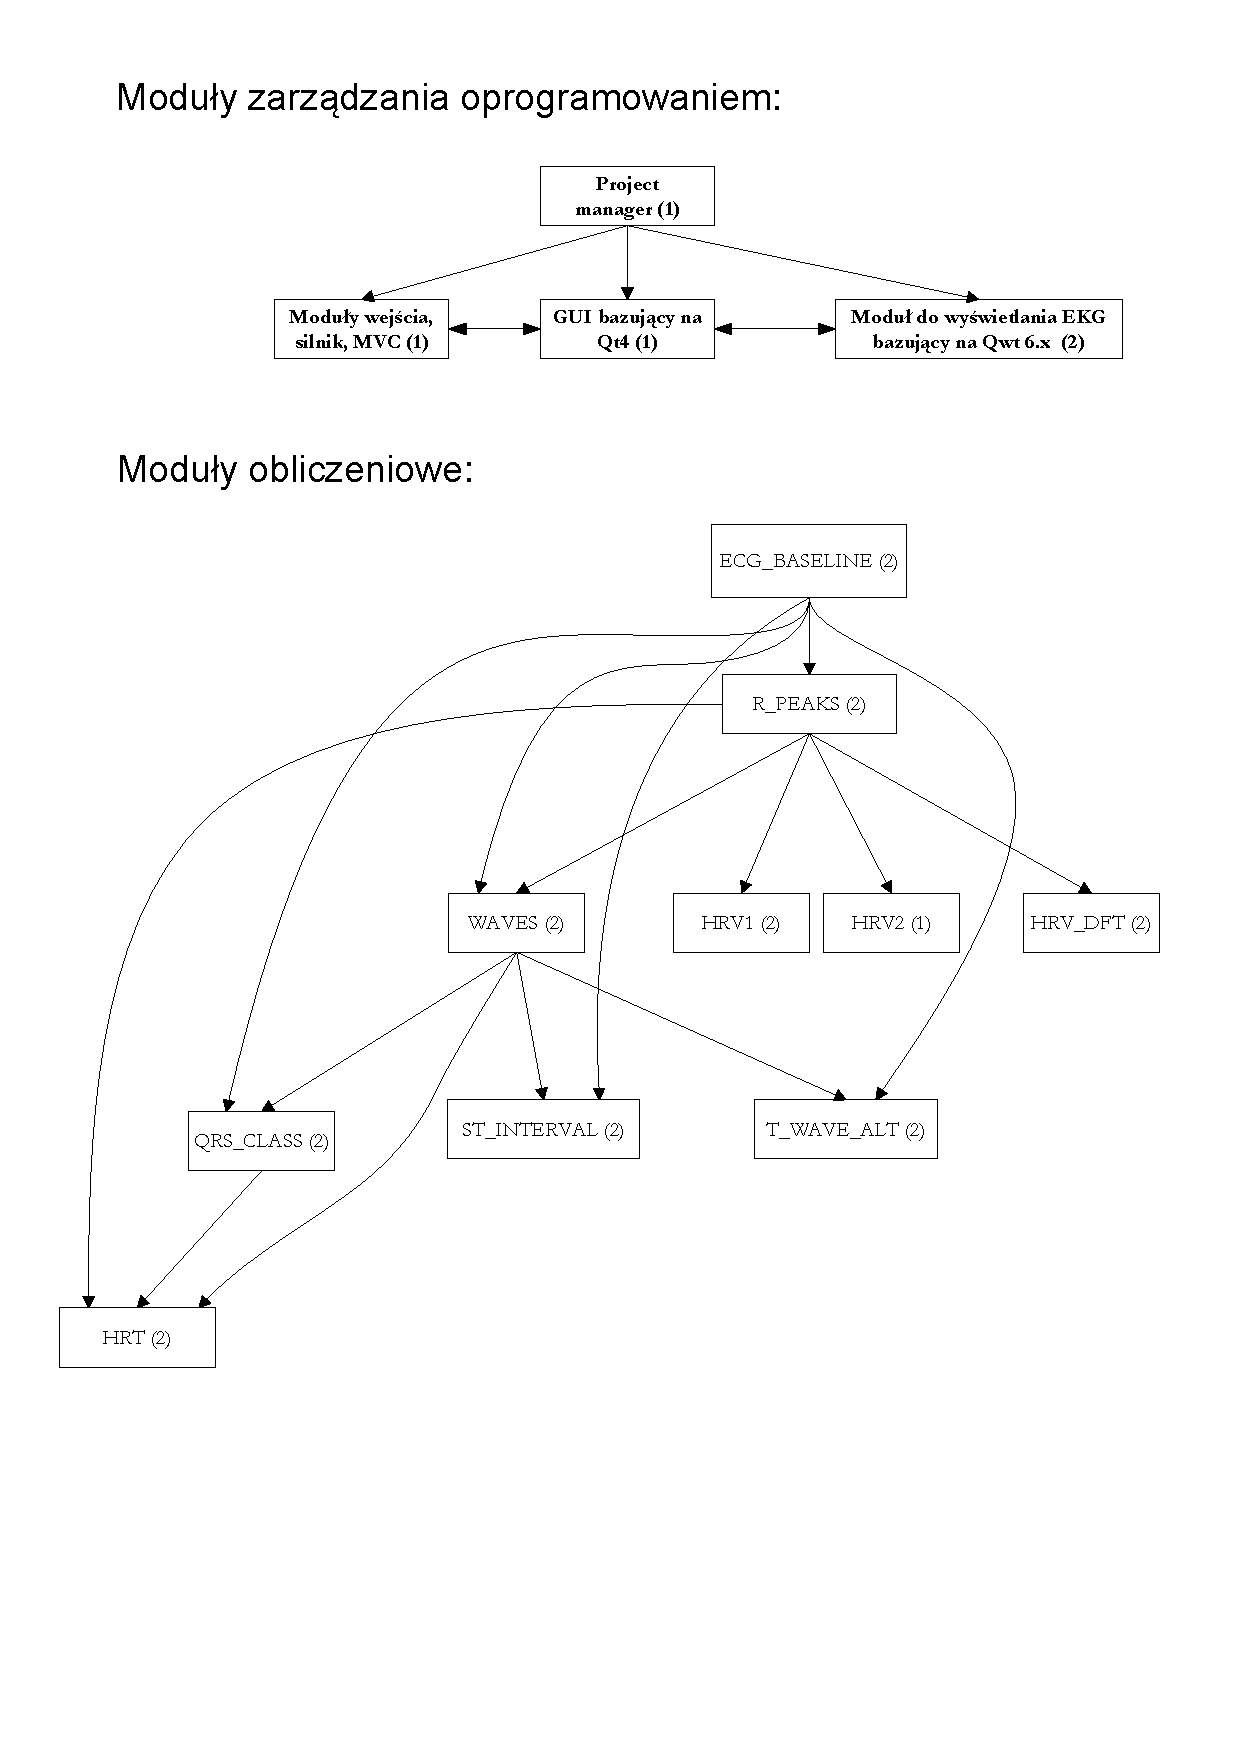
\includegraphics[width=0.7\linewidth]{include/Projekt_zaleznosci}
  \label{fig:zaleznosci}
  \caption{Zależności pomiędzy modułami projektu.}
\end{figure}

\section{Specyfikacja techniczna rozwiązania}
\label{sec:techspec}

\subsection{Wykorzystane narzędzia}
\label{sec:tools}

Podczas realizacji projektu wykorzystywane były różne narzędzia do tworzenia i prototypowania rozwiązań. Wstępne projekty przygotowywane były w programie Matlab, zaś ostateczny kod powstawał w języku C++ (standard '03 z elementami standardu C++11 obsługiwanymi przez wspierane kompilatory).
Minimalne wymagania kompilacji projektu są następujące:
\begin{itemize}
  \item Jeden z kompilatorów:
  \begin{itemize}
    \item Microsoft Visual Studio 2010
    \item GCC 4.5
  \end{itemize}
  \item Biblioteki:
  \begin{itemize}
    \item Boost 1.51
    \item Qt 4.8
    \item Qwt 6.01
    \item gsl 1.15
    \item WFDB 10.5.16 (zawarta w źródłach projektu)
    \item FFTW 3.3.2
  \end{itemize}
\end{itemize}

Do wersjonowania i śledzenia błędów wykorzystywaliśmy platformę Github wraz z rozproszonym systemem kontroli wersji Git. Posiada on zaawansowane możliwości wspierające pracę grupową nad projektem, co szczególnie przydaje się, gdy liczba osób jest duża.

\subsection{Projekt systemu}
\label{sec:sys_proj}

Program został wykonany w architekturze MVC -- istnieje ścisły podział na część wyświetlającą interfejs użytkownika, moduły przetwarzania sygnału oraz kontroler łączący te dwa elementy, co obrazuje diagram pakietów \ref{fig:package_diagram}. Zastosowano obiektowe podejście przy projektowaniu hierarchii klas realizujących przetwarzanie (rys. \ref{fig:class_diagram}), umożliwiające bezproblemową wymianę implementacji dowolnego modułu na inną.

\begin{figure}[h!]
  \centering
  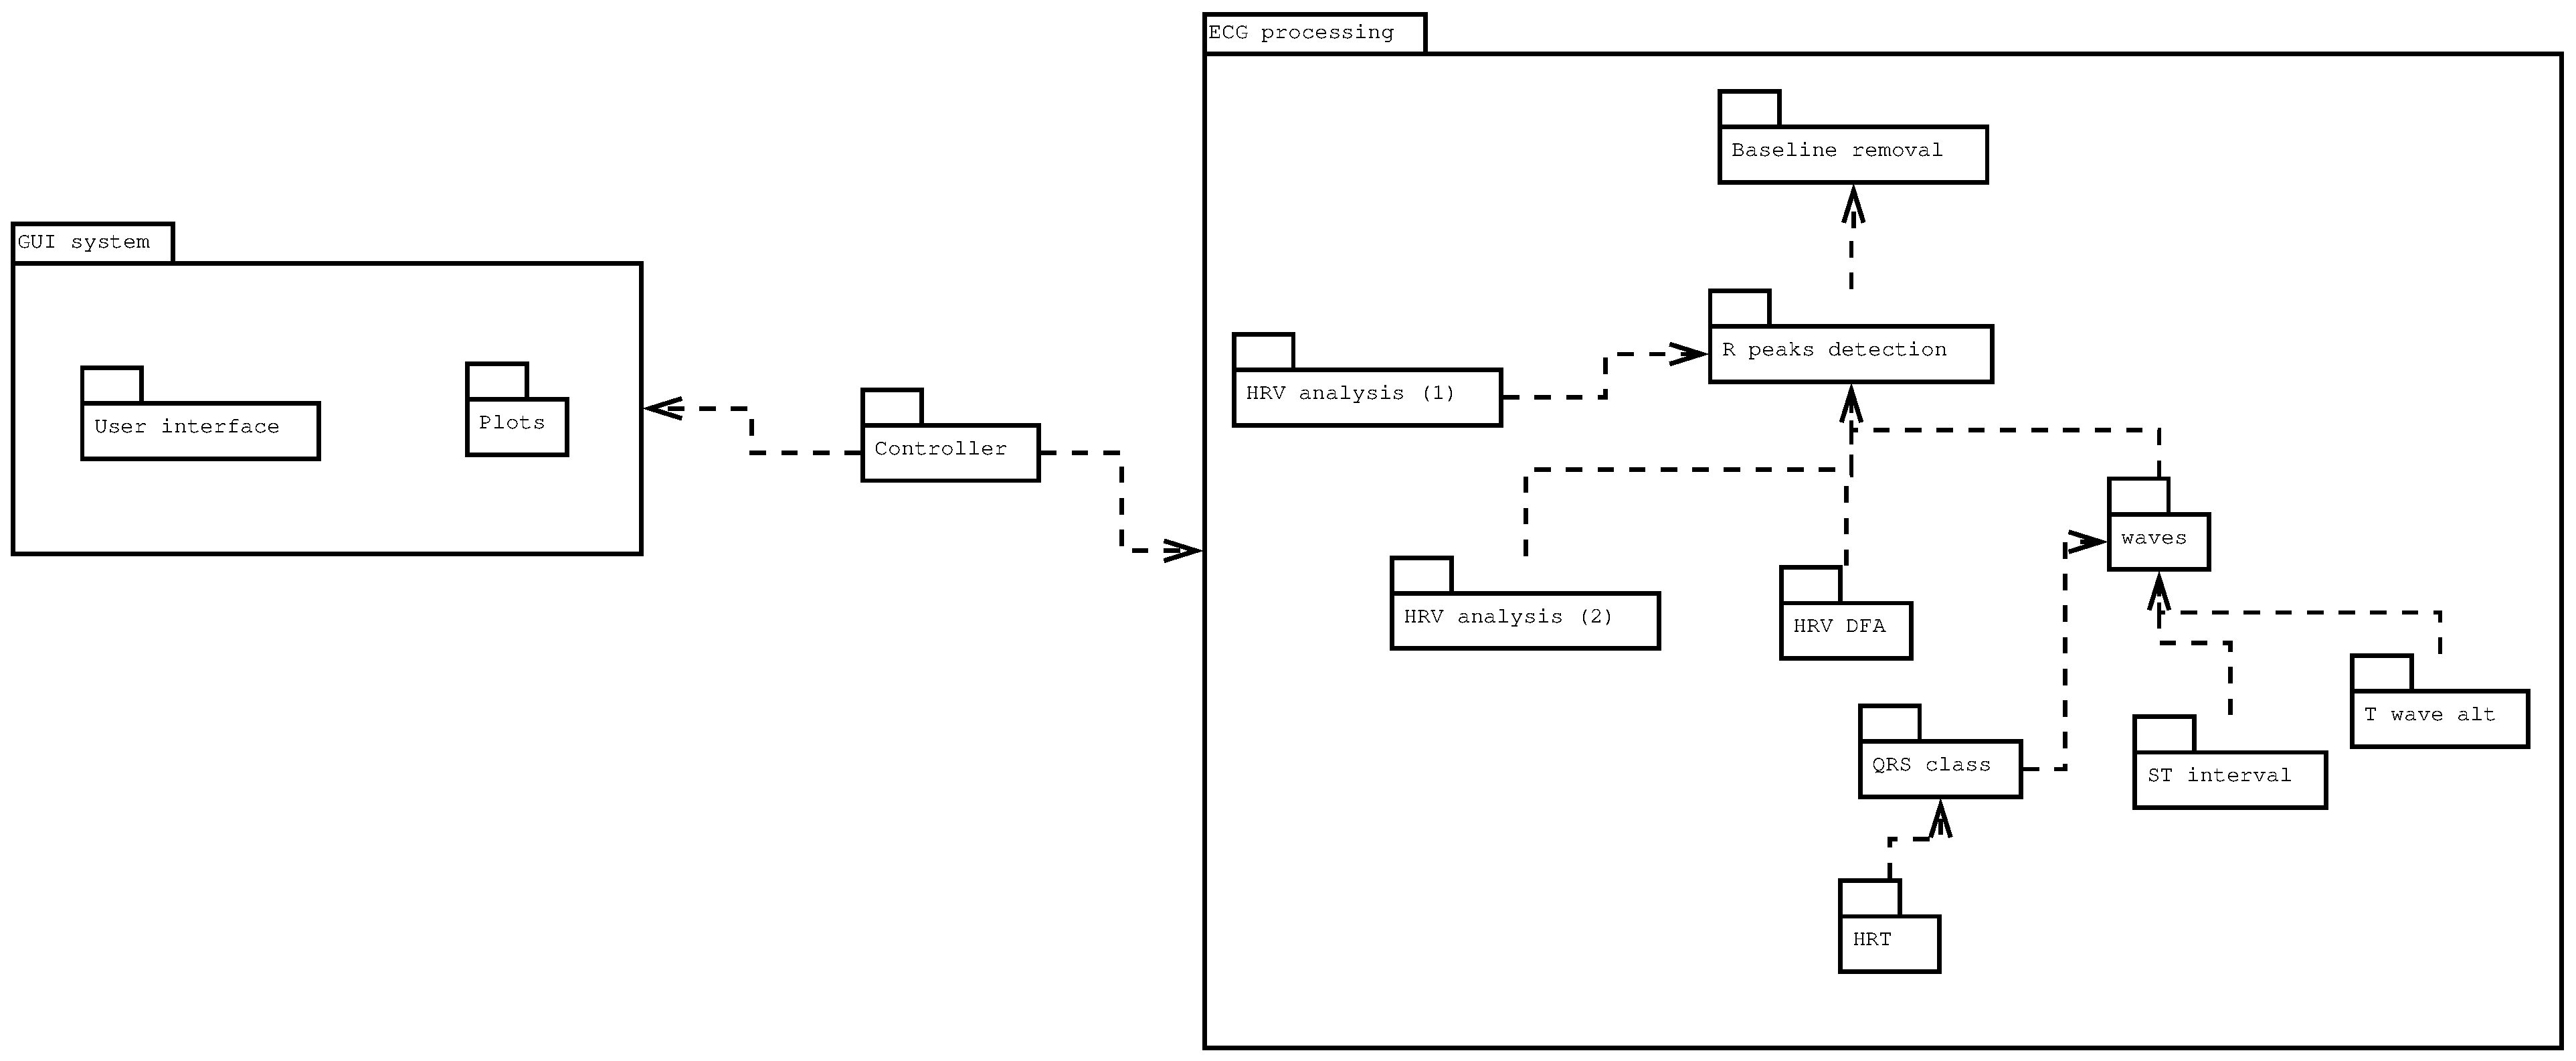
\includegraphics[width=\linewidth]{include/package_diagram}
  \label{fig:package_diagram}
  \caption{Diagram pakietów.}
\end{figure}

Samo przetwarzanie realizowane jest wielofazowo -- moduły przeliczane są sekwencyjnie na osobnym wątku niż wątek zdarzeń GUI, co pozwala na zatrzymanie zbyt długo trwającej operacji. Zaimplementowano także mechanizm buforowania wyników, dzięki czemu przy zmianie parametrów pewnego modułu nie ma konieczności przeliczania wyników modułów wcześniejszych.

Cała aplikacja napisana jest jako samodzielny, wieloplatformowy program (rys. \ref{fig:deployment_diagram}) -- możliwa jest kompilacja pliku binarnego pod systemami Windows, Linux i MacOS X. Całe przetwarzanie wykonywane jest lokalnie, dzięki czemu nie jest wymagane połączenie z Internetem. Dzięki wybraniu licencji GPL v2+ projekt jest wolny i możliwy jest jego dalszy rozwój i kompilacja na nowe platformy.

\begin{figure}[h!]
  \centering
  \includegraphics[width=0.5\linewidth]{include/deployment_diagram}
  \label{fig:deployment_diagram}
  \caption{Diagram wdrożenia.}
\end{figure}

Diagram sekwencji przedstawiający sposób uruchamiania modułów jest przedstawiony na rys. \ref{fig:sequence_diagram}.

\begin{figure}[h!]
  \centering
  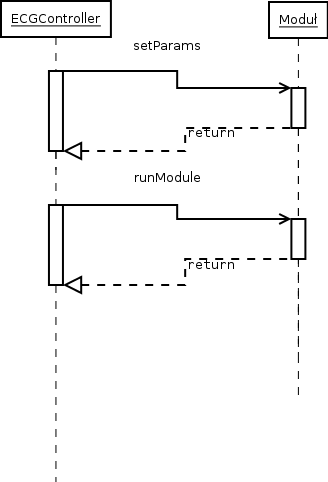
\includegraphics[width=0.5\linewidth]{include/sequence_diagram}
  \label{fig:sequence_diagram}
  \caption{Diagram sekwencji.}
\end{figure}

Diagram klas został przedstawiony na rys. \ref{fig:class_diagram}.

\begin{figure}[h!]
  \centering
  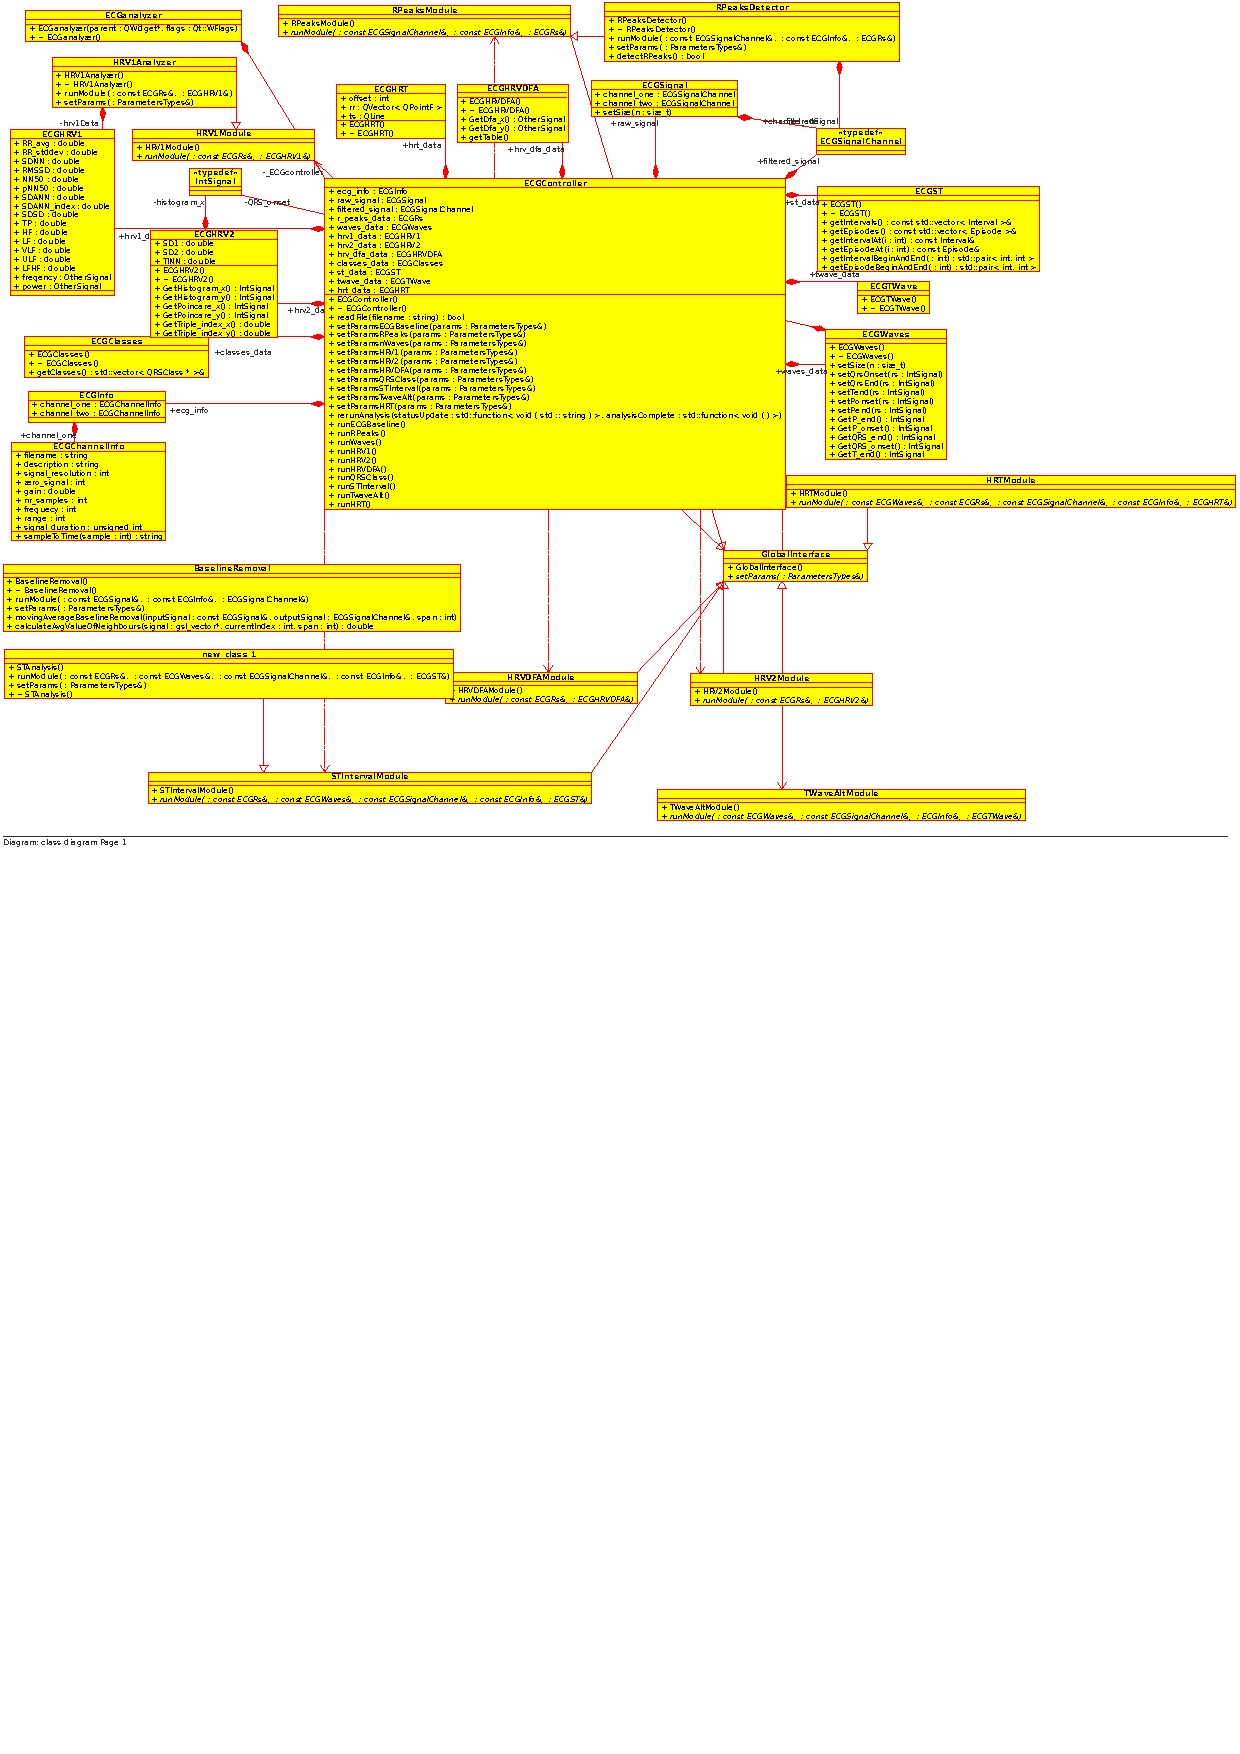
\includegraphics[width=0.9\linewidth]{include/class_diagram}
  \label{fig:class_diagram}
  \caption{Diagram klas.}
\end{figure}

\section{Opisy modułów}
\label{sec:mod}

\subsection{Usuwanie linii bazowej}
\label{sec:baseline}
Autorzy: Weronika Łabaj i Piotr Matuszkiewicz.

\subsubsection{Opis zadania}
\label{sec:baseline:desc}

\begin{description}
\item[Temat] Metody filtracji i detekcji izolinii w sygnale EKG
\item[Opis] Występujące zakłócenia sieciowe i mięśniowe, jak również falowanie linii izoelektrycznej w sygnale EKG niejednokrotnie uniemożliwiają właściwą i poprawną analizę sygnału. Celem projektu jest opracowanie i implementacja metod związanych filtracją i detekcją linii izoelektrycznej w sygnale EKG. W szczególności należy rozważyć:
  \begin{itemize}
  \item filtr Butterwortha,
  \item średnią kroczącą,
  \item metody nieadaptacyjne: filtr Savitzky-Golay’a
  \item metody atapdacyjne np. filtr Wienera, LMS
  \end{itemize}
\item[Dane] ciąg próbek sygnału EKG z bazy Physionet.org
\item[Szukane] moduł programu filtrujący sygnał EKG z zakłóceń sieciowych/mięśniowych oraz usuwający z sygnału falowanie linii izoelektrycznej przy wykorzystaniu różnych metod; w ostatecznym module programu będzie możliwość wyboru algorytmu filtrującego i usuwającego falowanie linii izoelektrycznej
\end{description}

\subsubsection{Badania literaturowe}
\label{sec:baseline:papers}

\subsubsection{Opis procedur i metod}
\label{sec:baseline:procs}

\subsubsection{Warunki testowania}
\label{sec:baseline:tests}

\subsubsection{Wyniki}
\label{sec:baseline:results}

\subsection{Wykrywanie załamków R}
\label{sec:Rs}

\subsection{Waves}
\label{sec:waves}

\subsection{HRV1}
\label{sec:hrv1}

\subsection{HRV2}
\label{sec:hrv2}

\subsection{HRV DFA}
\label{sec:hrvd_fa}

\subsection{Klasyfikacja zespołów QRS}
\label{sec:qrs_class}
Autorzy: Krzysztof Bębenek

\subsubsection{Opis zadania}
\label{sec:qrs_class:desc}

\begin{description}
\item[Temat] Metody detekcji morfologicznego pochodzenia zespołu QRS.
\item[Opis] Proces automatycznego klasyfikowania zespołów QRS należy do jednego z trudniejszych procesów podczas przetwarzania sygnałów EKG. Jest jednak on niezbędny w dalszych etapach analizy podczas których brane są pod uwagę tylko niepoprawne pobudzenia. Do prostych sposób oceny morfologi pobudzenia służą:
  \begin{itemize}
  \item współczynnik kształtu Malinowskiej,
  \item stosunek części ujemnej do dodatniej sygnału,
  \end{itemize}
\item[Dane] ciąg próbek przefiltrowanego sygnału EKG, wektory QRS\_onset oraz QRS\_end określające początek oraz koniec zespołu QRS
\item[Szukane] moduł programu klasyfikujący zespołu QRS na podstawie ich morfologii 
\end{description}

\subsubsection{Badania literaturowe}
\label{sec:qrs_class:papers}

\subsubsection{Opis procedur i metod}
\label{sec:qrs_class:procs}

\subsubsection{Warunki testowania}
\label{sec:qrs_class:tests}

\subsubsection{Wyniki}
\label{sec:qrs_class:results}



\subsection{ST interval}
\label{sec:st_interval}
Autorzy: Bartłomiej Bułat i Krzysztof Piekutowski.

\subsubsection{Opis zadania}
\label{sec:st_interval:desc}

\subsubsection{Badania literaturowe}
\label{sec:st_interval:papers}

\subsubsection{Opis procedur i metod}
\label{sec:st_interval:procs}

Główna funkcjonalność modułu znajduje się w klasie \verb|STAnalysis|. Klasa ta,
według przyjętego schematu rozszerza abstrakcyjny moduł analizy odcinka ST. W
tej klasie znajdują się drzewo klas prywatnych reprezentujących poszczególne
algorytmy analizy. W szczególności dwie klasy \verb|SimpleAnalizer| oraz
\verb|ComplexAnalizer|. Pierwsza klasa reprezentuje najprostszy algorytm
zaprezentowany w \cite[p.~155]{AUGUST1}, druga zaś implementuje lekko
zmodyfikowany algorytm opisany w \cite{SHEN1}.

%% TODO: mienić nazwę funkcji w programie
Lista i opis najważniejszych funkcji:

\begin{lstlisting}
void STAnalysis::SimpleAnalizer::analyse(const int it, const ECGRs& rpeaks,
  const ECGWaves& waves, const ECGSignalChannel& signal,
  const  ECGInfo& info, ECGST& output);
\end{lstlisting}

Funkcja analizująca załamek ST w zespole QRS numer \verb|it|. Wykorzystując
punkty sygnału obliczone we wcześniejszych modułach (tj. $QRS_{onset}$,
$QRS_{end}$ oraz $T_{end}$) oblicza koniec odcinka ST i wylicza jego parametry:
\begin{itemize}
  \item przesunięcie względem izolinii
  \item wartość nachylenia w stosunku do izolini
  \item długość odcinka ST
\end{itemize}
Uzywając wczesniej ustawionego parametru \verb|simple_thresh|, odcinek ST
określany jest jako ,,normalny'', ,,uniesiony'' lub ,,obniżony''.

Parametry:
\begin{itemize}
  \item \verb|const int it| -- numer badanego zespołu QRS, jako liczba
    porządkowa numerów próbek z tablicy załamków R.
  \item \verb|const ECGR& rpeaks| -- struktura zawierająca tablicę numerów
    próbek kolejnych załamków R
  \item \verb|const ECGEaves& waves| -- struktura zawierająca tablice
    przechowujące numery próbek punktów charakterystycznych kolejnych zespołów
    QRS: $P_{onset}$, $QRS_{onset}$, $QRS_{end}$ oraz $T_{end}$.
  \item \verb|const ECGSignalChanel& signal| -- jeden kanał odfiltrowanego
    sygnału z usuniętym przesunięciem izolinii.
  \item \verb|const ECGInfo& info| -- struktura zawierająca informacje o badanym
    sygnale EKG, m.in. częstotliwość.
  \item \verb|ECGST& output| -- parametr wyjściowy, struktura zawierająca
    tablice wszystkich interwałów ST wraz z ich parametrami, oraz tablice
    zarejestrowanych epizodów ST wraz z ich parametrami.
\end{itemize}

\begin{lstlisting}
void STAnalysis::ComplexAnalizer::analyse(const int it, const ECGRs& rpeaks,
  const ECGWaves& waves, const ECGSignalChannel& signal,
  const  ECGInfo& info, ECGST& output);
\end{lstlisting}

Funkcja analizująca załamek ST w zespole QRS numer \verb|it|. Wykorzystując
punkty sygnału obliczone we wcześniejszych modułach (tj. $QRS_{onset}$,
$QRS_{end}$ oraz $T_{end}$) oblicza koniec odcinka ST (wykorzystując bardziej
zaawansowane algorytmy od poprzedniej funkcji), a następnie oblicza jego parametry:
\begin{itemize}
  \item przesunięcie względem izolinii,
  \item wartość nachylenia w stosunku do izolinii,
  \item długość odcinka ST,
  \item klasyfikacja kształtu.
\end{itemize}
Używając wcześniej ustawionego parametru \verb|complex_thresh|, odcinek ST
określany jest jako ,,normalny'', ,,uniesiony'' lub ,,obniżony''. Algorytm
ocenia również to, czy załamek jest prosty czy zakrzywiony w oparciu o
wcześniej ustawiony parametr \verb|type_thresh|. Dla prostych odcinków określa
kierunek, czy narasta, opada czy jest poziomy. Do określenia tej cechy
wykorzystywany jest parametr \verb|slope_thresh|. Dla zakrzywiony odcinków ST
oceniana jest wypukłość krzywej. Szczegółowy opis działania znajduje się w
poprzednim rozdziale.

Parametry:
\begin{itemize}
  \item \verb|const int it| -- numer badanego zespołu QRS, jako liczba
    porządkowa numerów próbek z tablicy załamków R.
  \item \verb|const ECGR& rpeaks| -- struktura zawierająca tablicę numerów
    próbek kolejnych załamków R
  \item \verb|const ECGEaves& waves| -- struktura zawierające tablice
    przechowujące numery próbek punktów charakterystycznych kolejnych zespołów
    QRS: $P_{onset}$, $QRS_{onset}$, $QRS_{end}$ oraz $T_{end}$.
  \item \verb|const ECGSignalChanel& signal| -- jeden kanał odfiltrowanego
    sygnału z usuniętym przesunięciem izolinii.
  \item \verb|const ECGInfo& info| -- struktura zawierająca informacje o badanym
    sygnale EKG, m.in. częstotliwość.
  \item \verb|ECGST& output| -- parametr wyjściowy, struktura zawierająca
    tablice wszystkich interwałów ST wraz z ich parametrami, oraz tablice
    zarejestrowanych epizodów ST wraz z ich parametrami.
\end{itemize}

Funkcje pomocnicze klasy \verb|ComplexAnalizer|:

\begin{lstlisting}
int STAnalysis::ComplexAnalizer::getTPeak(const OtherSignal& sig,
  int from, int to);
\end{lstlisting}

Funkcja wyszukująca położenia punktu $T_{peak}$ na zadanym odcinku sygnału.
Początkiem wyszukiwania szczytu fali T jest zwykle punkt 20ms za punktem
$QRS_{end}$, a punktem końcowym jest koniec fali T. Funkcja wykorzystuje
dyskretną pochodną sygnału.

Parametry:
\begin{itemize}
  \item \verb|const OtherSignal& sig| - cały, odfiltrowany sygnał EKG
  \item \verb|int from| - numer próbki w której należy zacząć poszukiwania
  \item \verb|int to| - numer próbki w której należy skończyć poszukiwania
\end{itemize}


\begin{lstlisting}
std::pair<int, double> maxDistanceSample(const OtherSignal& signal, 
  int from, int to);
\end{lstlisting}

Funkcja szukająca numeru próbki najbardziej oddalonego od liniowej interpolacji
fragmentu sygnału miedzy dwoma punktami. Oprócz numeru próbki od początku
sygnału, zwracana jest wartość największej różnicy miedzy punktem sygnału, a
prostą interpolacji.

Parametry:
\begin{itemize}
  \item \verb|const OtherSignal& signal| - badany sygnał
  \item \verb|int from| - numer próbki będącej początkiem interesującego
    fragmentu sygnału, równocześnie, pierwszy punkt interpolacji liniowej.
  \item \verb|int to| - numer próbki będącej końcem interesującego fragmentu
    sygnału, równocześnie, drugi punkt interpolacji
\end{itemize}

\begin{lstlisting}
std::pair<int, int> overBelowSamples(const OtherSignal& signal,
  int from, int to);
\end{lstlisting}

Funkcja obliczająca ilość próbek ponad i poniżej prostej interpolującej sygnał
miedzy dwoma punktami. Funkcja wykorzystywana jest do określenia wypukłości
odcinka ST.

Parametry:
\begin{itemize}
  \item \verb|const OtherSignal& signal| - badany sygnał
  \item \verb|int from| - numer próbki będącej początkiem interesującego
    fragmentu sygnału, równocześnie, pierwszy punkt interpolacji liniowej.
  \item \verb|int to| - numer próbki będącej końcem interesującego fragmentu
    sygnału, równocześnie, drugi punkt interpolacji
\end{itemize}

\subsubsection{Warunki testowania}
\label{sec:st_interval:tests}

\subsubsection{Wyniki}
\label{sec:st_interval:results}

\subsection{T wave alt}
\label{sec:t_wave_alt}

\subsection{HRT}
\label{sec:hrt}

\bibliographystyle{plain}
\bibliography{report}
\end{document}
